% This file was created by tikzplotlib v0.8.7.
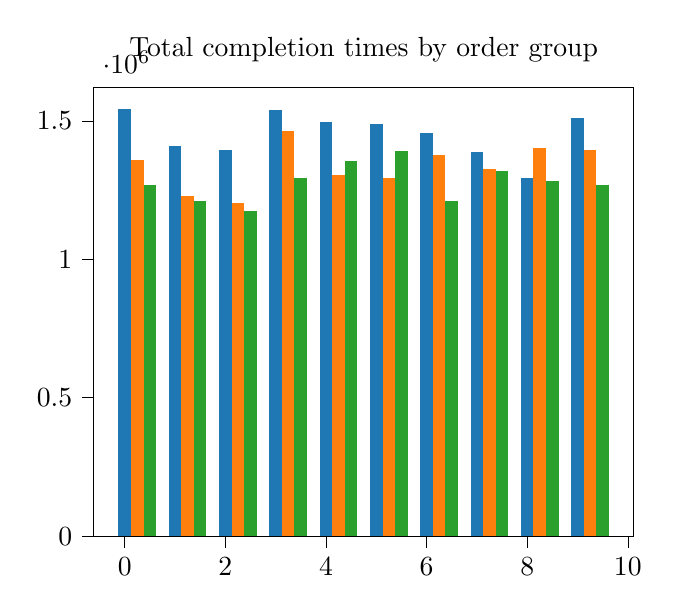
\begin{tikzpicture}

\definecolor{color0}{rgb}{0.12156862745098,0.466666666666667,0.705882352941177}
\definecolor{color1}{rgb}{1,0.498039215686275,0.0549019607843137}
\definecolor{color2}{rgb}{0.172549019607843,0.627450980392157,0.172549019607843}

\begin{axis}[
legend cell align={left},
legend style={fill opacity=0.8, draw opacity=1, text opacity=1, at={(0.03,0.97)}, anchor=north west, draw=white!80.0!black},
tick align=outside,
tick pos=left,
title={Total completion times by order group},
x grid style={white!69.01960784313725!black},
xmin=-0.6125, xmax=10.1125,
xtick style={color=black},
y grid style={white!69.01960784313725!black},
ymin=0, ymax=1619184,
ytick style={color=black}
]
\draw[fill=color0,draw opacity=0] (axis cs:-0.125,0) rectangle (axis cs:0.125,1542080);
\draw[fill=color0,draw opacity=0] (axis cs:0.875,0) rectangle (axis cs:1.125,1408896);
\draw[fill=color0,draw opacity=0] (axis cs:1.875,0) rectangle (axis cs:2.125,1394176);
\draw[fill=color0,draw opacity=0] (axis cs:2.875,0) rectangle (axis cs:3.125,1537568);
\draw[fill=color0,draw opacity=0] (axis cs:3.875,0) rectangle (axis cs:4.125,1496704);
\draw[fill=color0,draw opacity=0] (axis cs:4.875,0) rectangle (axis cs:5.125,1489568);
\draw[fill=color0,draw opacity=0] (axis cs:5.875,0) rectangle (axis cs:6.125,1457696);
\draw[fill=color0,draw opacity=0] (axis cs:6.875,0) rectangle (axis cs:7.125,1388608);
\draw[fill=color0,draw opacity=0] (axis cs:7.875,0) rectangle (axis cs:8.125,1294592);
\draw[fill=color0,draw opacity=0] (axis cs:8.875,0) rectangle (axis cs:9.125,1511904);
\draw[fill=color1,draw opacity=0] (axis cs:0.125,0) rectangle (axis cs:0.375,1357408);
\draw[fill=color1,draw opacity=0] (axis cs:1.125,0) rectangle (axis cs:1.375,1230336);
\draw[fill=color1,draw opacity=0] (axis cs:2.125,0) rectangle (axis cs:2.375,1203392);
\draw[fill=color1,draw opacity=0] (axis cs:3.125,0) rectangle (axis cs:3.375,1463552);
\draw[fill=color1,draw opacity=0] (axis cs:4.125,0) rectangle (axis cs:4.375,1303008);
\draw[fill=color1,draw opacity=0] (axis cs:5.125,0) rectangle (axis cs:5.375,1292192);
\draw[fill=color1,draw opacity=0] (axis cs:6.125,0) rectangle (axis cs:6.375,1375488);
\draw[fill=color1,draw opacity=0] (axis cs:7.125,0) rectangle (axis cs:7.375,1326080);
\draw[fill=color1,draw opacity=0] (axis cs:8.125,0) rectangle (axis cs:8.375,1403392);
\draw[fill=color1,draw opacity=0] (axis cs:9.125,0) rectangle (axis cs:9.375,1394304);
\draw[fill=color2,draw opacity=0] (axis cs:0.375,0) rectangle (axis cs:0.625,1267008);
\draw[fill=color2,draw opacity=0] (axis cs:1.375,0) rectangle (axis cs:1.625,1208960);
\draw[fill=color2,draw opacity=0] (axis cs:2.375,0) rectangle (axis cs:2.625,1173056);
\draw[fill=color2,draw opacity=0] (axis cs:3.375,0) rectangle (axis cs:3.625,1293344);
\draw[fill=color2,draw opacity=0] (axis cs:4.375,0) rectangle (axis cs:4.625,1356384);
\draw[fill=color2,draw opacity=0] (axis cs:5.375,0) rectangle (axis cs:5.625,1392544);
\draw[fill=color2,draw opacity=0] (axis cs:6.375,0) rectangle (axis cs:6.625,1212160);
\draw[fill=color2,draw opacity=0] (axis cs:7.375,0) rectangle (axis cs:7.625,1317184);
\draw[fill=color2,draw opacity=0] (axis cs:8.375,0) rectangle (axis cs:8.625,1281632);
\draw[fill=color2,draw opacity=0] (axis cs:9.375,0) rectangle (axis cs:9.625,1268064);
\end{axis}

\end{tikzpicture}
